\subsection{Overview}

In the following, a brief overview of the system's architecture is given in order to introduce the reader to the general structure of the system, highlighting the tasks separation.

The logic architecture of the system is composed of \textbf{three layer}. Each layer represents a distinct aspect of the system. These distinct aspects are the main tasks for which the system is design for. Each task is accomplished by a set of logically related functionalities, contained into one and only one of the logic layer. The communication between adjacent layers ties the logic architecture of the system. 

\begin{itemize}
	\item \textbf{Presentation layer}: where the datas are used, processed and converted into a usable form.
	\item \textbf{Logic layer}: where the whole logic of the system take place.
	\item \textbf{Data layer}: where the functionalities for data management live.
\end{itemize}

From a physical point of view, the system is layered in \textbf{four levels}, or \textit{tiers}. Each tier represents a physical computational node where the system's components are placed, according to their functionalities. Each tier is separated from the other and can communicate between themselves.

\begin{itemize}
	\item \textbf{Client tier}: layer containing the software components usable from the client to access to the system's functionalities and use the data requested.
	\item \textbf{Web server tier}: layer containing the components design for the processing of requests and responses.
	\item \textbf{Application tier}: layer containing the components created to implement and support the business logic.
	\item \textbf{Data tier}: layer containing software components for access and management of data.
\end{itemize}

\begin{figure}[H]
	\centerline{
		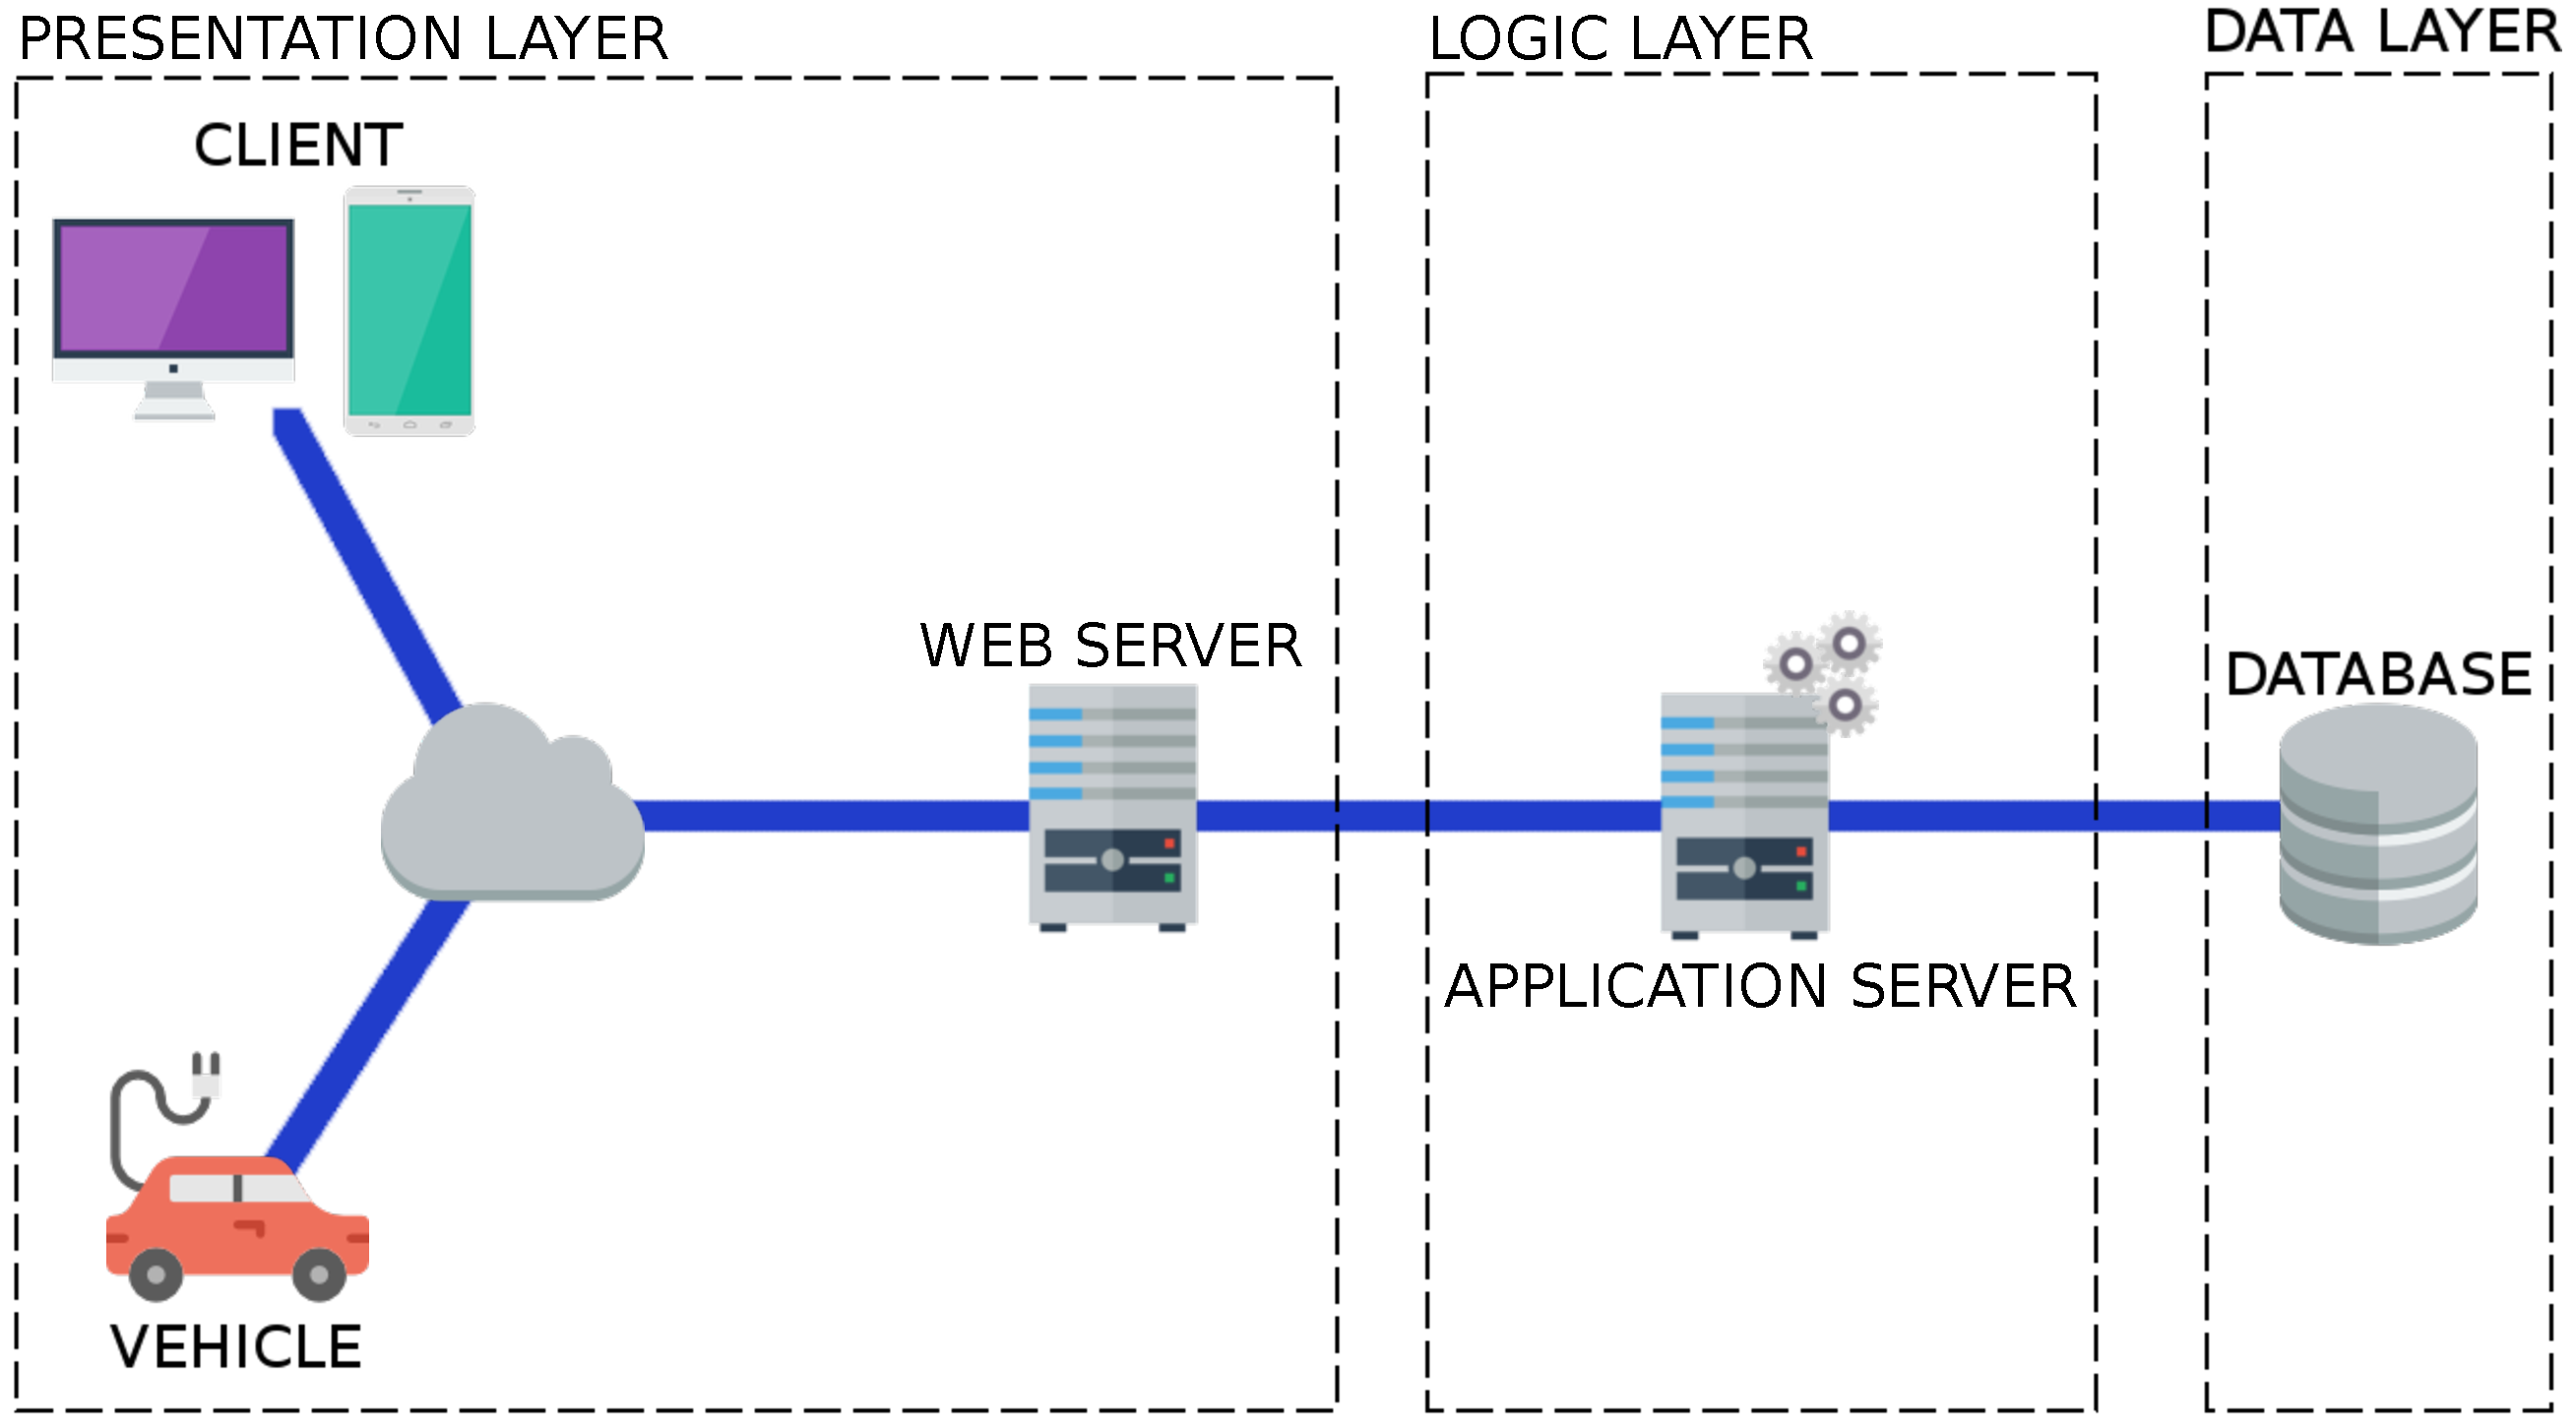
\includegraphics[width=350px]{../Datas/images/PEhla.pdf}
	}	
	\caption{Architecture's division in layers}
		\label{fig:PEhla}
\end{figure}

In order to design and, in the end, develop a highly scalable, flexible, easy to expande and easy to maintain system some design principles has been taken in consideration during the process of identification of the functional components composing the system to be:

\begin{itemize}
	\item \textbf{High Cohesion.}
	\item \textbf{Loose Coupling.}
	\item \textbf{High level of abstraction.}
	\item \textbf{Separation of concerns.}
\end{itemize}

Since the environment where the system will be deployed is a highly concurrent context, with requests coming from a large and heterogeneous set of devices, and the workload generated is generally unpredictable, some design choices oriented to increase the performance of the system has been considered.
Such choices are deeply discussed in \textit{\nameref{sec:selected-styles-patterns}} section, describing the motivation for their choice and how they are used.

Design choices not regarding performances, i.e. System's security, are shown and explained in \textit{\nameref{sec:other-design-decisions}}.
